\documentclass[tikz, border=1pt]{standalone}

% \usetikzlibrary{calc}
\usetikzlibrary{math}

\begin{document}
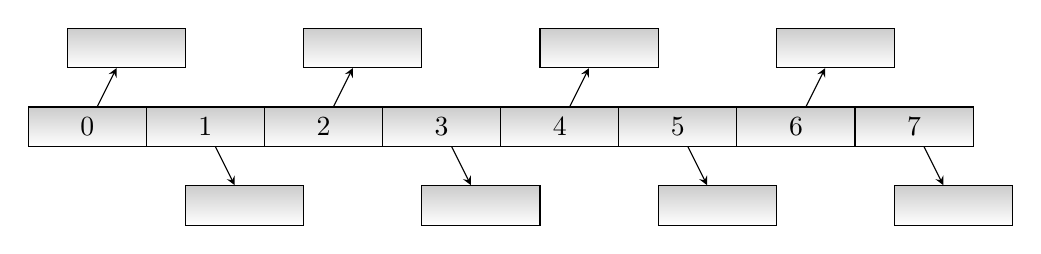
\begin{tikzpicture}
   [
      >=stealth,
      item/.style={rectangle, draw, inner sep=0pt, minimum width=1.5cm, minimum
      height=5mm, top color=black!20, bottom color=white}
   ]
   \foreach \i in {0,...,7}
      \node[item] (address\i) at (1.5*\i,1) {\i};

   \foreach \i in {0,2,...,6} {
      \node[item] (object\i) at (1.5*\i+0.5,2) {};
      \tikzmath{
         int \j;
         \j = \i+1;
      }
      \node[item] (object\j) at ({1.5*\j+0.5},0) {};
   }

   \foreach \i in {0,...,7}
      \draw[->] (address\i) -- (object\i);
\end{tikzpicture}
\end{document}

% vim: ft=tex tw=90 sts=-1 sw=3 et fdm=marker
